\documentclass[a4paper,11pt,eval]{nsi} 
\usepackage{pifont}
\usepackage{fontawesome5}

%\pagestyle{empty}


\newcounter{exoNum}
\setcounter{exoNum}{0}
%
\newcommand{\exo}[1]
{
	\addtocounter{exoNum}{1}
	{\titlefont\color{UGLiBlue}\Large Exercice\ \theexoNum\ \normalsize{#1}}\smallskip	
}



\begin{document}



\textcolor{UGLiBlue}{Vendredi 06/12/2024}\\
\classe{\premiere spé}
\titre{Evaluation-bilan 3}
\maketitle
\begin{center}
	Calculatrice autorisée. Toutes les réponses doivent être justifiées.
\end{center}

\vspace{1cm}

\exo{}\bareme{5 pts}
\begin{enumerate}
    %\item On définit la suite $(u_n)$ par : pour tout $n\in\N, \quad u_n=1-3n$.\\
    %Calculer les quatre premiers termes de la suite $(u_n)$.
    \item On définit la suite $(u_n)$ par : $\left\{
	\begin{array}{llll}
		u_0 & = & -2 &\\
		u_{n+1} & = & u_n + \dfrac{2}{3} & \text{pour tout } n\in\N.\\
	\end{array}
	\right. $
    \begin{enumalph}
        \item Calculer les trois premiers termes de la suite $(u_n)$.
        \item Calculer les variations de la suite $(u_n)$.
    \end{enumalph}
    \carreauxseyes{16}{14.4}
	\newpage
    \item On définit la suite $(v_n)$ par : pour tout $n\in\N, \quad v_n=4\times 9^n$.
    \begin{enumalph}
        \item Calculer les 3 premiers termes de $(v_n)$.
        \item Justifier que pour tout $n\in\N,\ v_n>0$.
        \item En calculant $\dfrac{v_{n+1}}{v_n}$ pour $n\in\N$, déterminer les variations de la suite $(v_n)$.\\
    \end{enumalph}  
	\carreauxseyes{16}{14.4}
\end{enumerate}

\vspace*{1cm}
\exo{}\bareme{6 pts}\\
Soit $(w_n)$ la suite définie par $w_n=n^2+6n+4$ pour tout $n\in \N$.
\begin{enumerate}
	\item 	Soit $f:x\mapsto x^2+6x+4$ définie sur $\R$.\\
	\'Ecrire $f$ sous forme canonique et dresser le tableau de variation de $f$.
	\item 	En déduire les variations de $(w_n)$.
	\item	À partir de quel rang $(w_n)$ dépasse-t-elle la valeur 100 ?\\
\end{enumerate}

\carreauxseyes{16.8}{25.6}


\vspace*{.5cm}

\exo{}\bareme{5 pts}\\
On considère la succession de figures suivantes :
\begin{center}
	\begin{tikzpicture}[scale=0.46]
		\draw[fill=UGLiBlue] (0,0) circle (0.5cm);
		\draw[fill=UGLiBlue] (1.2,0) circle (0.5cm);
		\draw[fill=UGLiBlue] (0,1.2) circle (0.5cm);
		\draw[fill=UGLiBlue] (1.2,1.2) circle (0.5cm);
		\draw[] (-0.8,-1.5) node[right]{Figure 1} ;
		
		\draw[fill=UGLiBlue] (5,0) circle (0.5cm);
		\draw[fill=UGLiBlue] (6.2,0) circle (0.5cm);
		\draw[fill=UGLiBlue] (5,1.2) circle (0.5cm);
		\draw[fill=UGLiBlue] (6.2,1.2) circle (0.5cm);
		\draw[fill=UGLiBlue] (7.4,1.2) circle (0.5cm);
		\draw[fill=UGLiBlue] (6.2,2.4) circle (0.5cm);
		\draw[fill=UGLiBlue] (7.4,2.4) circle (0.5cm);
		\draw[] (4.2,-1.5) node[right]{Figure 2} ;
		
		\draw[fill=UGLiBlue] (11.2,0) circle (0.5cm);
		\draw[fill=UGLiBlue] (12.4,0) circle (0.5cm);
		\draw[fill=UGLiBlue] (11.2,1.2) circle (0.5cm);
		\draw[fill=UGLiBlue] (12.4,1.2) circle (0.5cm);
		\draw[fill=UGLiBlue] (13.6,1.2) circle (0.5cm);
		\draw[fill=UGLiBlue] (12.4,2.4) circle (0.5cm);
		\draw[fill=UGLiBlue] (13.6,2.4) circle (0.5cm);
		\draw[fill=UGLiBlue] (14.8,2.4) circle (0.5cm);
		\draw[fill=UGLiBlue] (13.6,3.6) circle (0.5cm);
		\draw[fill=UGLiBlue] (14.8,3.6) circle (0.5cm);
		\draw[] (10.4,-1.5) node[right]{Figure 3} ;
		
	\end{tikzpicture}
\end{center}
On note $a_n$ le nombre de jetons nécessaires à la construction de la figure $n$ où $n\in\N^*$.
\begin{enumerate}
	\item 	Donner les valeurs de $a_1, a_2$ et  $a_3$.
	\item 	Donner une relation de récurrence permettant de définir la suite $(a_n)$.
	\item	Conjecturer une formule explicite du terme général de la suite $(a_n)$.
	\item	En supposant exacte la conjecture émise à la question \textbf{3}, déterminer :
	\begin{enumalph}
		\item 	la valeur de $a_{30}$ ;
		\item 	la plus grande figure que l'on puisse construire avec 200 jetons.\\
	\end{enumalph}
\end{enumerate}

\carreauxseyes{16.8}{14.4}\\
\carreauxseyes{16.8}{10.4}\\

\vspace*{.5cm}

\exo{}\bareme{3 pts}\\
\dleft{9cm}{
    Soit $(q_n)$ la suite définie par
$$\quad \left\{
\begin{array}{llll}
	q_0 & = & 1 & \\ 
	q_{n+1} & = &f(q_n) & \text{pour tout } n\in\N\\
\end{array}
\right. $$
La courbe représentative de $f$ sur l'intervalle $[0\ ; 8]$ est tracée dans le repère ci-contre.

\begin{enumerate}
	\item 	Représenter graphiquement les cinq premiers termes de $(q_n)$.
	\item 	\'Emettre une conjecture sur la limite de cette suite.
\end{enumerate}
}
{
    \def\xmin{-1} \def\ymin{-1}\def\xmax{8}\def\ymax{9}
	\def\F{8/(1+\x)+1}
	\begin{tikzpicture}[scale=.8]
		\clip (\xmin,\ymin) rectangle (\xmax,\ymax);
		\draw[fill = white] (\xmin,\ymin) rectangle (\xmax,\ymax);
		\repereal{\xmin}{\ymin}{\xmax}{\ymax}
		\draw[thick,color=gray,domain=\xmin:\xmax,smooth,variable=\x] plot ({\x},{\x});	
		\draw[thick,domain=-.9:\xmax,smooth,variable=\x] plot ({\x},{\F});	
	\end{tikzpicture}\
}
\carreauxseyes{16.8}{4.8}

\newpage
\exo{}\bareme{4 pts}\\
\dleft{11.8cm}{
La pyrale est une chenille invasive qui s'attaque aux buis (un arbuste à petites feuilles).\\
Un massif des Pyrénées en est victime depuis quelques années. 
}
{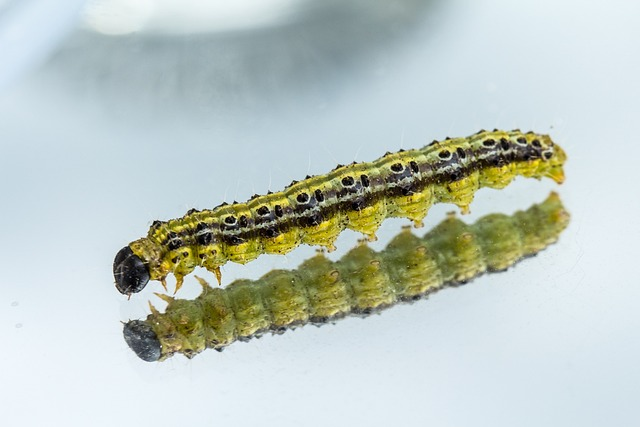
\includegraphics[width=4.5cm]{caterpillar.jpg}}
Les agents de l'ONF (Office National des Forêts) estiment que, chaque année, cette chenille fait disparaître 15 \% des buis de ce massif.\\
On compte 75 000 pieds de buis en 2024. 
\begin{enumerate}
    \item Si rien n'est fait pour lutter contre cette chenille, quelle conjecture peut-on émettre quant au nombre de buis dans ce massif à long terme ?
    \item Les agents de l'ONF replantent 3000 plants de buis chaque année pour compenser les dégats.
    \begin{enumalph}
        \item Calculer le nombre de buis dans ce massif en 2025 et en 2026.
        \item On note $b_n$ le nombre de buis dans ce massif en 2024$+n$.\\
        Expliquer la formule de récurrence $\quad b_{n+1}=0,85\ b_n+3000\quad$ pour tout entier naturel $n$.
        \item \faCalculator \hspace*{.1cm} Quelle conjecture peut-on émettre quant au nombre de buis dans ce massif à long terme ? \textit{On pourra utilier la calculatrice pour formuler une conjecture.}
    \end{enumalph}
\end{enumerate}
\carreauxseyes{16.8}{14.4}
\end{document}